\subsection{Model parametrization}
\label{sec:param}
\subsubsection{Sea surface wind stress}


Equation X in Y20 is,

\begin{equation}
 |\tau| = C_d(|U|) \cdot U^2
 \label{eq:tau}
 \end{equation}

 It is unclear whether this increase or decreases at high wind speeds
 \cite{powell2003reduced, donelan2004limiting}. Y20~\cite{ZannaPreprint} speculates that $C_d$ may naturally continue
to increase with windspeed, making Eq.~\ref{eq:tau} closer to cubic.

We can make sense of Equation~\ref{eq:tau} by analogy to the pressure of an ideal
gas caused by the impact of a molecule of speed $u$, where one factor of
$u$ comes from the probability of collision, and one from the momentum
exchanged during each collision.

\subsubsection{Sea surface wind induced heat transfer}
The uncertainty in this parametrization of this may be an explanation as to why there are
not enough Safir-Simpson category 4 and 5 in models~\cite{emanuel2005divine}.



    \begin{figure}
            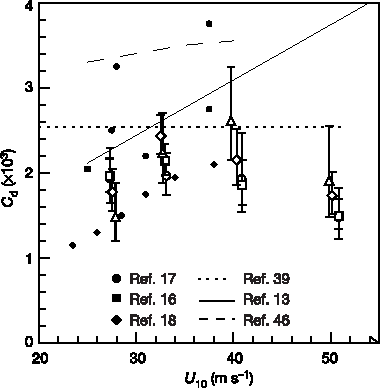
\includegraphics[width=1\linewidth]{images/example-images/cd.pdf}
                \caption{Fig. 3c from Powell 2003~\cite{powell2003reduced},
                 where they suggested that at high wind speeds $c_d$ decreases.}
    \end{figure}
\begin{figure}[htb!]
    \centering
    \includegraphics[width=1\linewidth]{../surge/plots/cd_finder.pdf}
    \caption{ Extracting $C_d$ from data.
    $ r_p = 0.9774 \pm 0.001,\;\; p<10^{-300}$\\
    $ m = 0.0383 \pm 0.0001 $ kg$^{0.5}$ m$^{-1.5}$\\
    $\implies  c_d = 0.001467 \pm 0.000008$ kg m$^{-3}$
    % error estimated from differences in output between test/training year,
    % measured regression error in either year much smaller than this.
    % The error is propogated using the \texttt{python3.uncertanties} package}
    There might be a theoretical limit~\cite{donelan2004limiting}.
    }
    %\label{fig:}
\end{figure}


Equation 4 in \cite{zou2017observation},

\begin{equation}
Q_{H}=\rho c_{p} C_{H} U\left(\theta-\theta_{0}\right),
\end{equation}


maintenance of tropical cyclones depend exclusively
 on self-induced heat transfer from the ocean through this route.
